\chapter{Experiments and results}
This section discusses the performance of the proposed scheme on various network parameter. For experiments and simulation Network Simulator 2.35 is used. Here in the given section, we first give a brief description of simulator used, the network configuration and its parameters. Next we analyze the impact of our proposed system to the conventional baseline system. In the given process, we compare the proposed and baseline systems over performance metrics like packet loss, end-to-end delay and network lifetime.
\section{Simulator}
Network Simulator 2,version 2.35 is used to model the network environment. Due to the factors such as flexibility and modular nature, NS-2 can be used in various problem domains such as:
\begin{enumerate}
    \item Modelling of wired and wireless communication networks.
    \item Specifying network protocols and simulating their behaviour.
    \item Modeling of queueing networks.
\end{enumerate}
Network Simulator Version 2, widely known as NS2, is an event driven simulation tool that is useful in studying the dynamic nature of communication networks. Simulation of wired as well as wireless network functions and protocols (e.g., routing algorithms, TCP, UDP) can be done using NS2. 
\par
 Figure 4.1 below shows the basic architecture of NS2. NS2 provides users with an executable command ns which takes on input argument, the name of a Tcl simulation scripting file. Users are feeding the name of a Tcl simulation script (which sets up a simulation) as an input argument of an NS2 executable command ns. In most cases, a simulation trace file is created, and is used to plot graph and/or to create animation.
 \begin{figure}[h!]
    \centering
    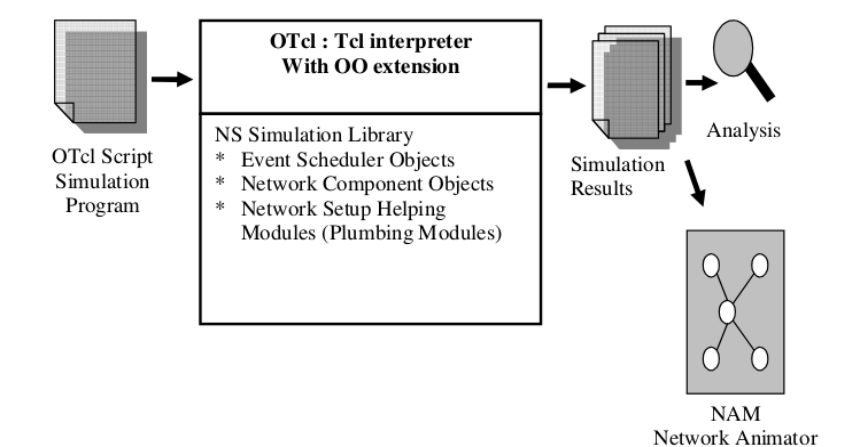
\includegraphics[height=6cm, width=13cm]{Thesis/figs/NS2archi.png}
    \caption{Architecture of NS2}
    \label{fig:my_label}
\end{figure}
 \par 
NS2 consists of two key languages: C++ and Object-oriented Tool Command Language (OTcl). While the C++ defines the internal mechanism (i.e.,a back end) of the simulation objects, the OTcl sets up simulation by assembling and configuring the objects as well as scheduling discrete events (i.e.,a front end). The C++ and the OTcl are linked together using TclCL. Mapped to a C++ object, variables in the OTcl domains are sometimes referred to as handles. Conceptually, a handle (e.g., n as a Node handle) is just a string (e.g.,o10) in the OTcl domain, and does not contain any functionality. Instead, the functionality(e.g., receiving a packet) is defined in the mapped C++ object (e.g., of class Connector). In the OTcl domain, a handle acts as a front end which interacts with users and other OTcl objects. It may defines its own procedures and variables to facilitate the interaction. 
 \par
 NS2 provides a large number of built in C++ objects. It is advisable to use these C++ objects to set up a simulation using a Tcl simulation script. However, sometimes we may find these objects insufficient. In this case, we need to develop our own C++ objects, and use a OTcl configuration interface to put together these objects. After simulation, NS2 outputs either text-based or animation-based simulation results. To interpret these results graphically and interactively, tools such as NAM (Network AniMator) and XGraph are used.
 \section{Simulation setup}
 The WSN simulated comprises of deployed sensor nodes transmitting the sensed information back to the sink. Table 4.1 shows the parameter used in NS2 simulations. The number of nodes are 10-50.In the simulations, packet length is set to 100 bytes and the routing protocol used is AODV i.e. Ad Hoc On-Demand Distance Vector Routing protocol.  
\begin{table}[h!]
\begin{center}
\caption{Parameters used in NS2 simulation}
\begin{tabular}{ |p{3.2cm}|p{3.5cm}|  }
\hline
\multicolumn{2}{|c|}{Experimental Setup} \\
\hline
Parameters & Value  \\
\hline
Number of nodes & 10-50   \\
Source rate &  200 Kbps  \\
Packet size &  100 bytes \\
Traffic type & UDP \\
Queuing schemes &  DropTail, RED, Proposed scheme\\
Buffer size & 150 packets\\
Routing protocol &  AODV\\
MAC protocol &  802.11  \\
Simulation time  & 200 time-step  \\
Initial Energy per node & 25 Joules \\
Threshold energy & 0.5 Joules\\
\hline
\end{tabular}
\end{center}
\end{table}
 The whole operation is done on IEEE.802.11 module provided. We have made the changes as per the need in the codes of the different sub-modules required at the network layer. 
 \subsection{Scenario 1:}
 This network scenario comprises of the following:
 \begin{enumerate}
     \item Network of 50 nodes are deployed. Node 6 has been assigned as sink where each source tries to send their information respectively.
     \item The network is simulated firstly with the conventional approach and then the proposed scheme.
     \item The results are obtained by averaging the results from ten independent simulation runs for network size with varied number of nodes.
      \item Inside the network, nodes 9,10 and 13 transmits the correlated data to the sink.
      \item The total number of packets sent from the sources is approximately $2 \times 10^{5}$ packets per source in each simulation run.
 \end{enumerate}
\begin{figure}[h!]
    \centering
    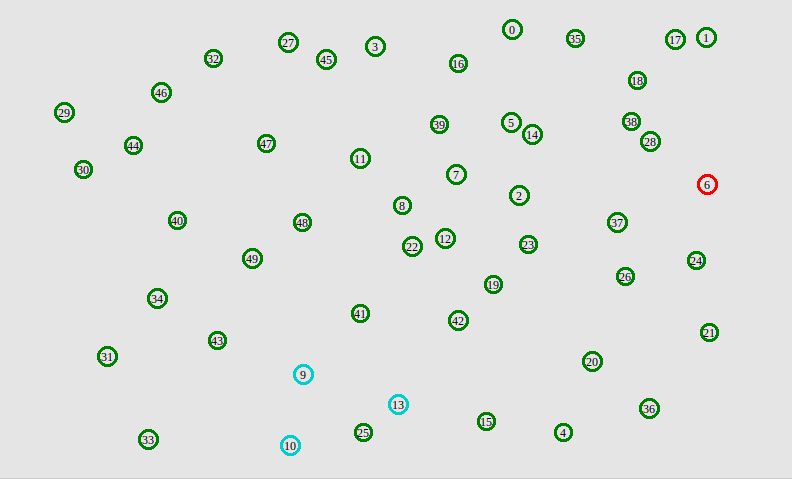
\includegraphics[scale=0.45]{Thesis/figs/scenario1.png}
    \caption{Simulation scenario 1 }
    \label{fig:my_label}
\end{figure} 
 \subsection{Scenario 2:}
 This scenario is made more prone to spatial redundant transmission by adding nodes 22,12 and 19 sending correlated data.
 \begin{figure}[h!]
    \centering
    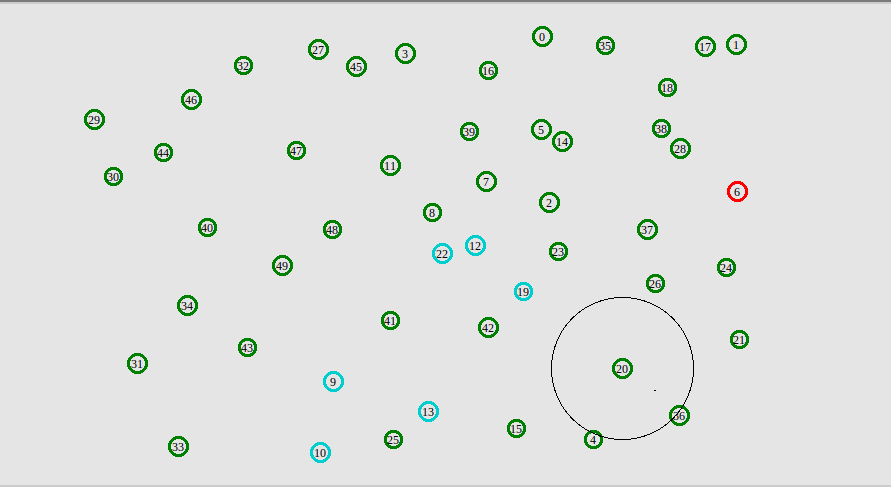
\includegraphics[scale=0.45]{Thesis/figs/scenario2.png}
    \caption{Simulation scenario 2 }
    \label{fig:my_label}
\end{figure} 
 \subsection{Scenario 3:}
 This scenario comprises node 3 and node 44 to transmit the redundant information.
\section{Results and Discussions}
In order to prove that the proposed approach performs better than the conventional approach, we have compared various performance metrics in the following sections.
\subsection{Packet Drop Ratio}
Table 4.4 shows the packet drop ratio and average end-to-end delay for Drop Tail, queuing schemes Random Early Detection and Proposed Scheme.
Packet drop ratio(PDR) is calculated by the formula specified in Equation 4.1: \\
\begin{equation}
    PDR = \frac{Dropped packets}{Generated packets}
\end{equation}
Figure 4.4 presents the frequency of packet losses for the Drop Tail and two queuing schemes. The packet loss ratio represents the ratio of the number of lost packets to the total number of sent packets.
\begin{table}[h!]
\begin{center}
\begin{tabular}{|p{3.5cm}|p{3.5cm}|p{4.2cm}|  }
\hline
Queuing Scheme & Packet drop ratio & End-to-End delay(ms.) \\
\hline
Drop Tail & 0.239 & 15.05\\
\hline
Random Early Detection & 0.221 & 11.951   \\
\hline
Proposed Scheme & 0.069 & 10.117 \\

\hline
\end{tabular}
\caption{Packet loss and average end-to-end delay}
\end{center}
\end{table}
The buffer size was selected according to the delay limitations. The
delay and network congestion are directly proportional to the buffer size and source rate,respectively. The results presented in the following are obtained by averaging results from ten independent simulation runs.
\begin{figure}[h!]
    \centering
    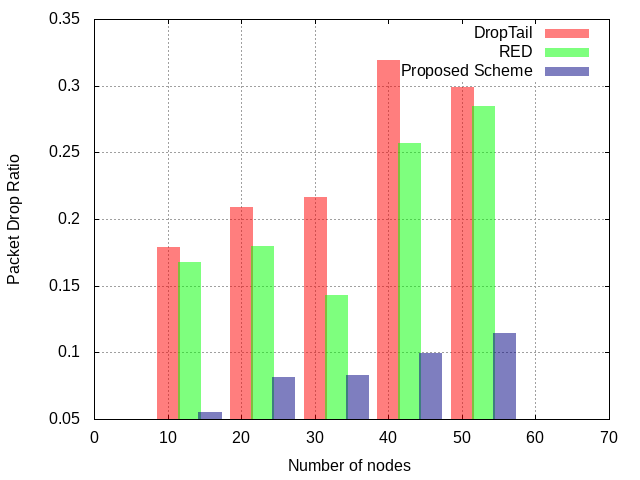
\includegraphics[scale=0.8]{Thesis/figs/outcome2.png}
    \caption{Probability of packet loss versus number of nodes}
    \label{fig:my_label}
\end{figure}
The packet drop ratio in case of proposed scheme doesn't vary much over the network size. The reason is the packets carrying the same sensing data and within the time difference of less than $10^{-6}$ seconds are labelled as redundant packets, given the drop probability of 1. \\
The simulation for the topology in figure 4.5, where node 36 receives the same data at the same time from two different nodes 9 and 13. In such a scenario, the data packets are dropped having redundant information.  
\begin{figure}[h!]
    \centering
    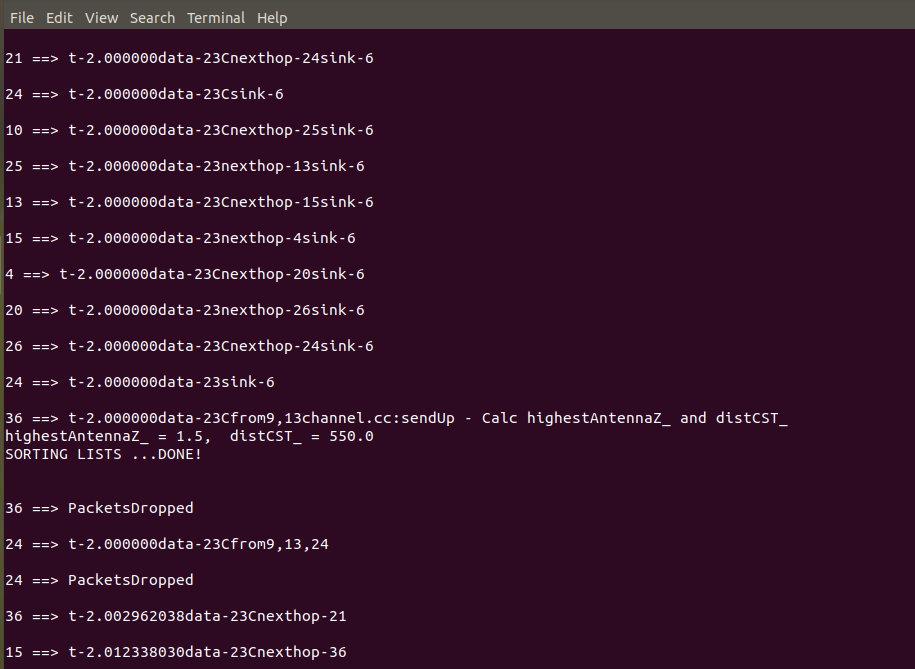
\includegraphics[scale=0.5]{Thesis/figs/screen.png}
    \caption{Simulation Scenario}
    \label{fig:my_label}
\end{figure}
\subsection{Average End-to-end delay}
\vspace{0.5cm}
The average end-to-end delay is shown in the figure 4.6. The end-to-end delay is defined between the time a packet is generated at the sensor to the time it is received by the sink. The proposed scheme provides significantly lower average end-to-end delay compared to RED for various network sizes. The reason for such observation is when the proposed scheme drops the redundant packets from the buffer, the average number of packets in the buffer gets reduced. Following from Equation 3.11, the reduction in the number of packets occupying the buffer space,eventually reduces the average delay experienced by the non-redundant nodes in the network.    
\begin{figure}[h!]
    \centering
    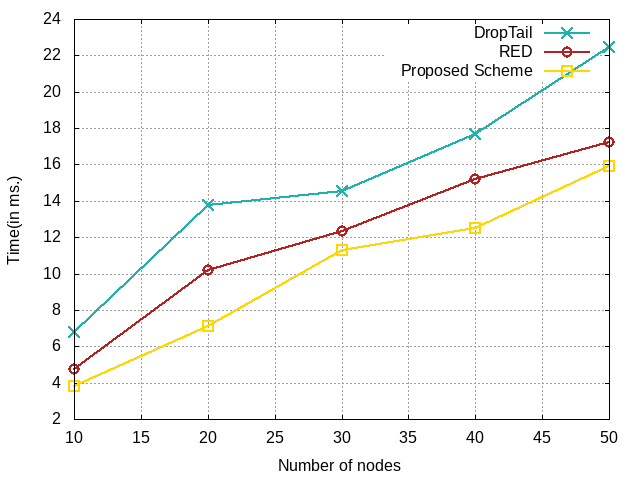
\includegraphics[scale=0.8]{Thesis/figs/delay1.png}
    \caption{Average End-to-end delay}
    \label{fig:my_label}
\end{figure}
\subsection{Network Lifetime}
Network lifetime is perhaps the most important metric for the evaluation of sensor networks. Of course, in a resource constrained environment, the consumption of every limited resource must be considered. However, network lifetime as a measure for energy consumption occupies the exceptional position that it forms an upper bound for the utility of the sensor network. 
\par
The network lifetime for the proposed scheme is given in figure 4.7. 
\begin{figure}[h!]
    \centering
    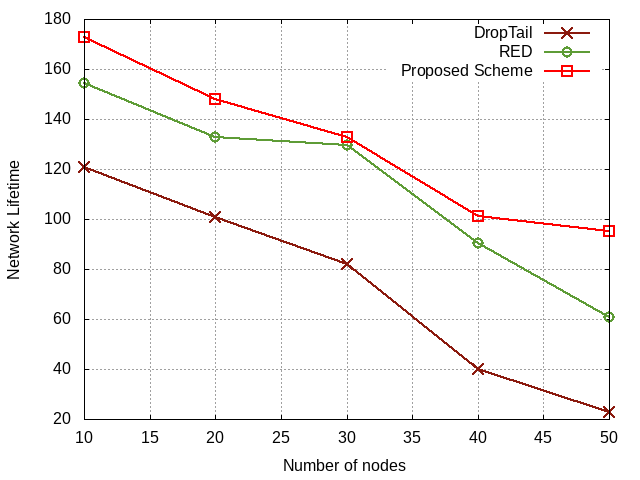
\includegraphics[scale=0.8]{Thesis/figs/lifetime.png}
    \caption{Network lifetime}
    \label{fig:my_label}
\end{figure}
\par
The initial energy provided to each node in the network is 25 Joules. The threshold set for the node energy is set to 0.5 Joules below which, it cannot receive or transmit in the network. In the figure, the proposed scheme have extended network lifetime for various network sizes as compared to the Drop Tail and RED mechanism. This is due to the reason that proposed scheme drops packets initially before the buffer at any node gets full, thereby reducing the occurrence of congestion. 
\section{Overall conclusion}
This chapter evaluates the performance of the proposed approach over various performance metrics. As shown the proposed mechanism successfully removes the redundant transmission taking place in the network. As a result, there is an significant improvement in the packet drop ratio in the network (about 69 percent). Network lifetime has been significantly approved than the baseline mechanisms. All these benefits aligned with the predicted mathematical calculation. However, average end-to-end delay didn't follow the same trend as other metrics. The improvement in end-to-end delay was compromised due to the reason that the additional amount of time was taken by the nodes in calculating the correlation among the packets as the traffic was increased. The forthcoming chapter concludes the whole thesis work and proposes future aspect regarding this work.